
\begin{figure*}
    \begin{minipage}[c][10cm][c]{0.5\textwidth}
        \centering
        \vspace*{\fill}
        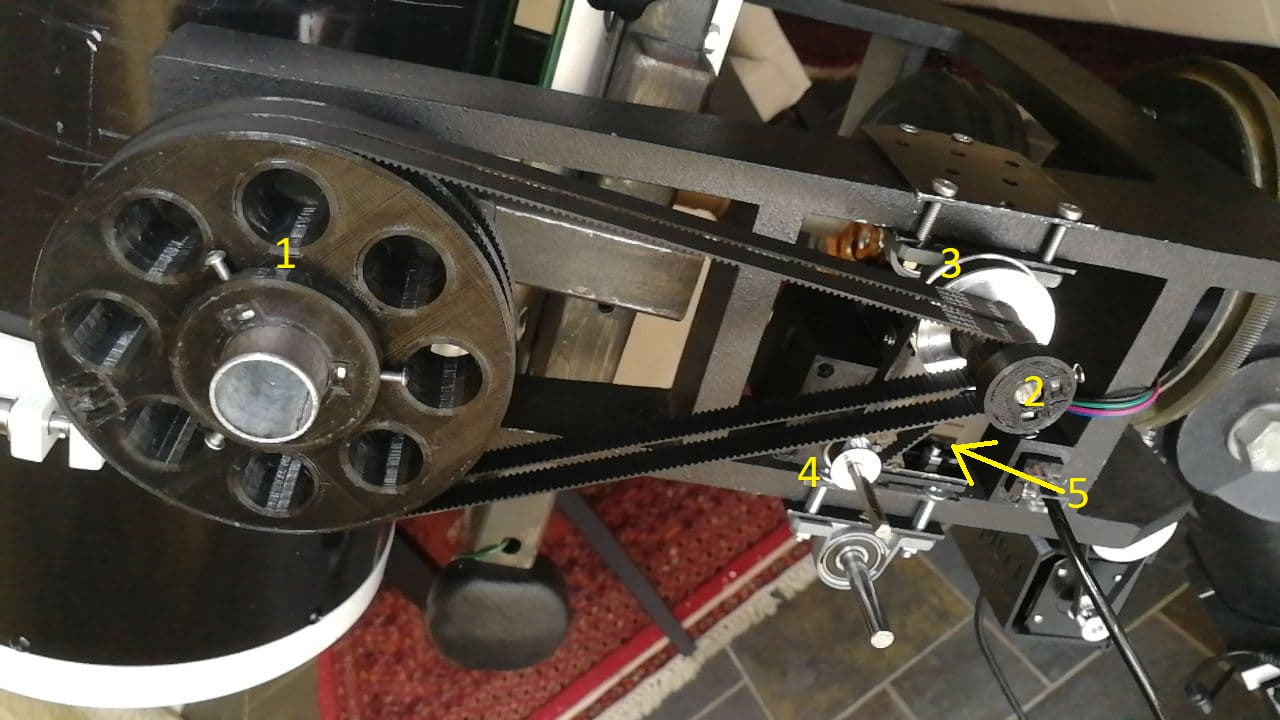
\includegraphics[height=4.5cm]{DEC-v3.jpg}
        \subcaption{DEC V1 mechanism.}
        \label{fig:DEC_mechanism_v3}
        
        \addtocounter{subfigure}{1}
        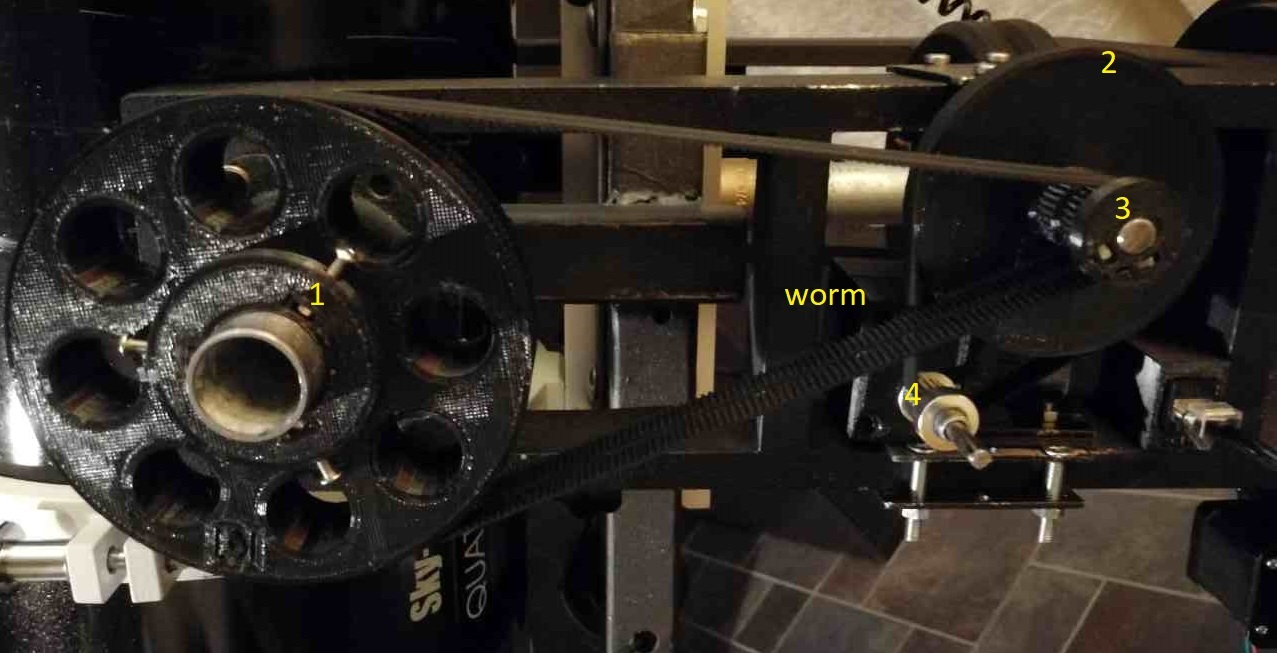
\includegraphics[height=4.5cm]{DEC-v4.jpg}
        \addtocounter{subfigure}{-2}
        \subcaption{DEC V1+ mechanism.}
        \label{fig:DEC_mechanism_v1p} 
    \end{minipage}
    \begin{minipage}[c][10cm][t]{0.5\textwidth}
        \vspace*{\fill}
        \centering
        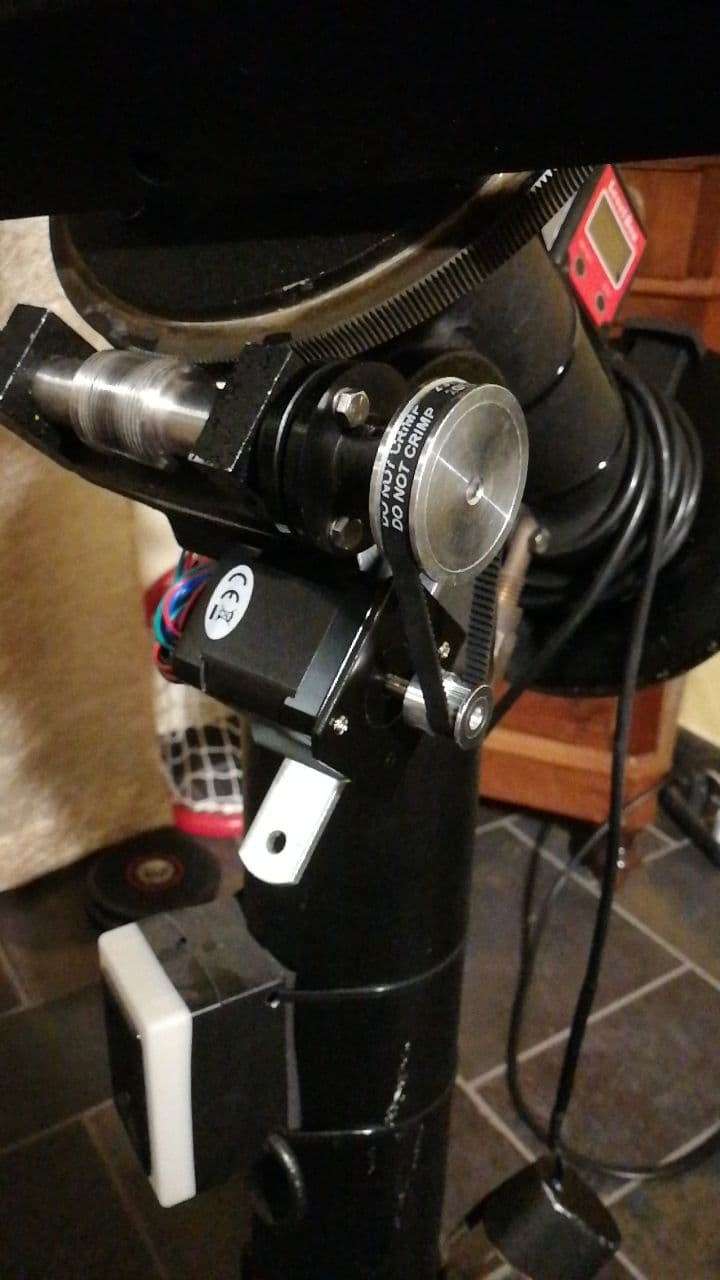
\includegraphics[height=9cm]{RA_motorization.jpg}
        \subcaption{RA mechanism.}
        \label{fig:RA_mechanization}
    \end{minipage}
    \caption{RA and two of the many versions of the DEC mechanization.}
    \label{fig:dec-versions}
\end{figure*}

\section{Mechanization}
\label{sec:mechanization}

% \begin{figure*}
%     \centering
%     \begin{subfigure}[t!]
%         {.3\textwidth}
%         \centering
%         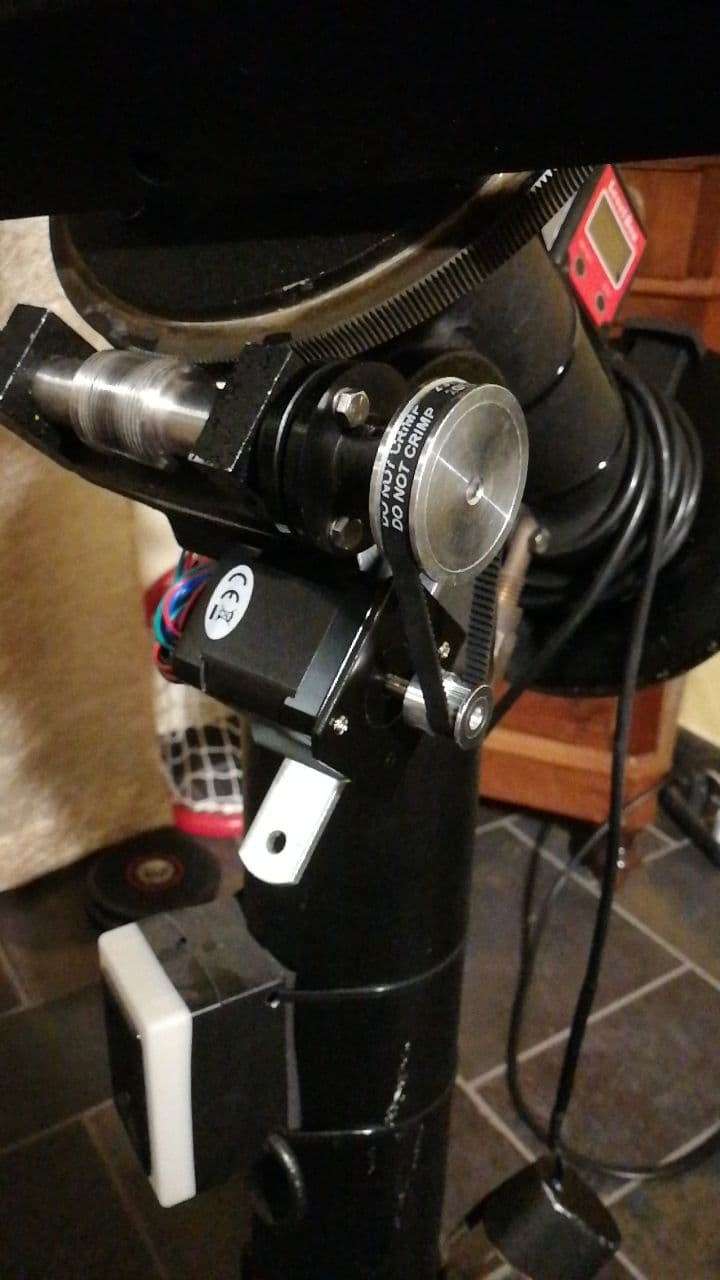
\includegraphics[scale=0.6]{RA_motorization.jpg}  
%         \captionof{figure}{Nema 17 stepper motor and gear adjustment.}
%         \label{fig:RA_mechanization}         
%     \end{subfigure}
%     \begin{subfigure}[t!]
%         {0.3\textwidth}
%         \centering
%         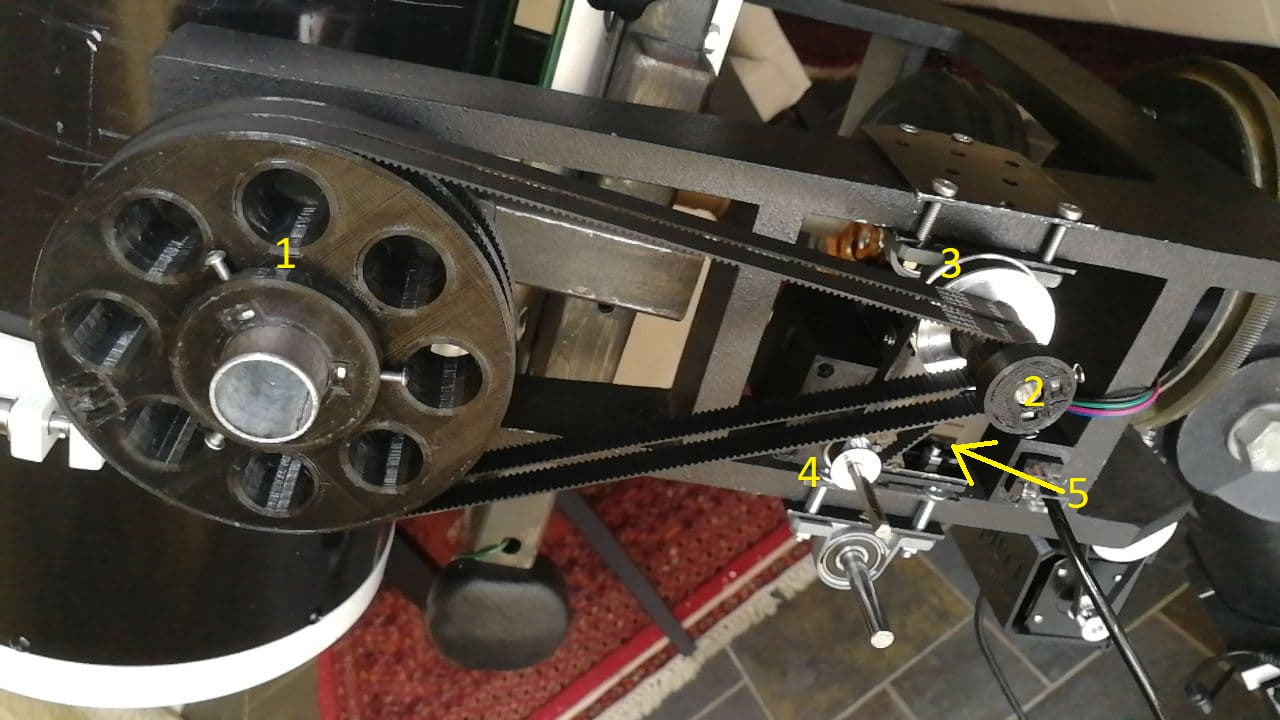
\includegraphics[scale=.6]{DEC-v3.jpg}
%         \caption{DEC V1 mechanism.}
%         \label{fig:DEC_mechanism_v3}
%     \end{subfigure}

%     \begin{subfigure}[t!]
%         {0.3\textwidth}
%         \centering
%         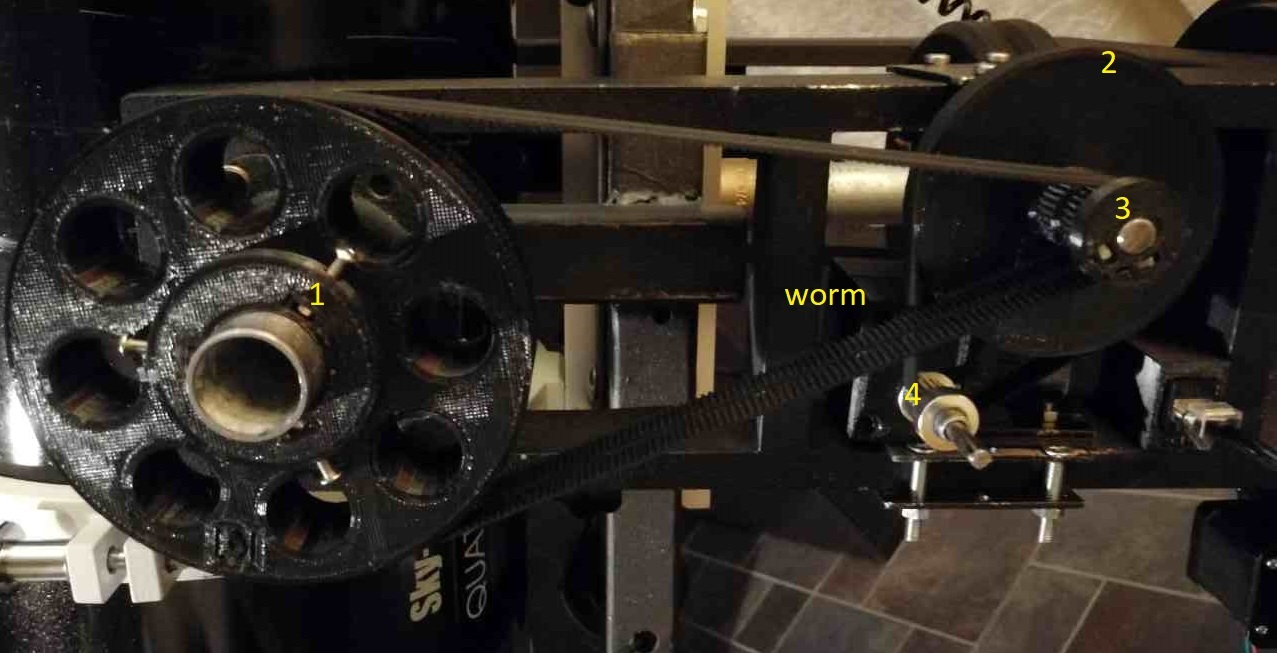
\includegraphics[scale=.25]{DEC-v4.jpg}
%         \caption{DEC V1+ mechanism.}
%         \label{fig:DEC_mechanism_v1p}
%     \end{subfigure}
%     \caption{RA and two of the many versions of the DEC mechanization.}
%     \label{fig:dec-versions}
% \end{figure*}

The motorization of the telescope passes through two mechanics adjustments:
\begin{enumerate}
    \item motorize the RA movement, exploiting the native tracker mechanism;
    \item motorize the DEC movement, which natively has no gears.
\end{enumerate}
Before entering in the details, we define the stepper motors used in the setup.

\subsection{Stepper motors}
In this subsection we write the specifics of the stepper motors used for the RA and DEC mechanization (for both we have used nema 17 motors) and the focuser (developed with a nema 11 stepper motor).

\subsection{RA motorization}
The telescope's mount has already a tracking mechanism motorized by a 3W synchronous motor.
So, in principle, it is only a matter of substitute this old motor, with a new programmable stepper motor.

The gears are composed by:
\begin{itemize}
    \item a 359 teeth stage (1 tooth for each degree, fantastic);
    \item an endless screw (worm) mounted on a shaft through a clutch.
\end{itemize}
Using this structure, for a continuous sky tracking, the elder motor would complete a round of the worm in 4 minutes.
Thus, this mechanism rotates the mount with the velocity of a degree in 4 minutes (which is the velocity of the sky moving away in the night).

We have reduced the ratio by a third adding two other gears (see figure \ref{fig:RA_mechanization}): 60 teeth gear positioned in the shaft and a 20 teeth gear on the motor shaft.
\\
\begin{minipage}{.4\textwidth}
    \centering
    \begin{tabular}{cc|c}
        ratio gear 1 & ratio gear 2 & total ratio \\
        \hline
        1/360 & 1/3 & 1/1080 \\
        \hline
    \end{tabular}
    \captionof{table}{Total reduction of RA mechanization.}
    \label{tab:RA_mechanization}
\end{minipage}
\\

We have choose to install a nema 17 stepper motor with the specifics in table \ref{tab:nema_17_specifics}

\subsection{DEC motorization}
The mechanization of the DEC axis was a bit more complicated since there was not a built-in gear to use.
We tried different versions.
A first successfully try was to exploit a stand-alone disk.
On the edge of the latter are present some ticks and grades: it was used a declination angle teller.

As told above, we have tried different configurations, but same stepper motor is used.

\subsubsection{DEC V1}
Using a 3D printer we have designed a double-belt gear.
Then, a 1/10 ratio is obtained using a worm gear and another 1/3 is obtained between the worm and the final gear.
The total reduction with all gear specifics is reported in table \ref{tab:DEC_gear_spec_v3}.
Figure \ref{fig:DEC_mechanism_v3} is a picture of the mechanism.
The precision of the mechanism is 
\[\delta_{th.}=0.28'',\quad \delta_{est.}=0.96''\]
where \(th.\) stands for theoretical and \(est.\) stands for estimated.

\begin{minipage}
    {0.5\textwidth}
    \textbf{DEC-V1 stages}\\
    \centering
    \begin{tabular}{cccccc}
        \hline
        Gear number & 1 & 2 & 3 & 4 & worm\\
        number of teeth & 180 & 30 & 60 & 20 & 10\\
        \hline
        total ratio & \(\sim \frac{1}{180}\) &&&
    \end{tabular}
    \captionof{table}{DEC mechanism's gear specifics.}
    \label{tab:DEC_gear_spec_v3}
\end{minipage}

\subsubsection{DEC V1+}
Starting from the DEC V1, we have designed a new gear to get a bigger reduction ratio (this is the reason for the +).
The total reduction with all gear specifics is reported in table \ref{tab:DEC_gear_spec_v1p}.
Figure \ref{fig:DEC_mechanism_v1p} is a picture of the mechanism.
The precision of the mechanism is 
\[\delta_{th.}=0.14'',\quad \delta_{est.}=0.48''\]
where \(th.\) stands for theoretical and \(est.\) stands for estimated.

\begin{minipage}
    {0.5\textwidth}
    \textbf{DEC-V1+ stages}\\
    \centering
    \begin{tabular}{cccccc}
        \hline
        Gear number & 1 & 2 & 3 & 4 & worm\\
        number of teeth & 180 & 30 & 120 & 20 & 10\\
        \hline
        total ratio & \(\sim \frac{1}{360}\) &&&
    \end{tabular}
    \captionof{table}{DEC mechanism's gear specifics.}
    \label{tab:DEC_gear_spec_v1p}
\end{minipage}

\subsection{Focuser motorization}
Another improvement is the motorization of the focuser.
Using a nema 11 stepper motor, we have created the motor supports and the gears using a 3D printer.
The reduction stage is 1/3, and the mechanism is visible in figure \ref{fig:focuser-box}.